% !TEX root = main.tex

\chapter{Conclusion and Future Perspectives}
\label{chap:conclusion}

The accurate parameterization of lithium-ion batteries is not merely a theoretical exercise in system identification; it is the foundational prerequisite for safe, efficient, and long-lasting operation of modern electric vehicles and grid energy storage systems. Across this report, the experimental, mathematical, and computational frameworks required to extract internal battery states and parameters—scaling from a single equivalent circuit branch to complex multi-cell pack topologies—have been systematically developed.

This concluding chapter synthesizes the methodologies presented in the preceding thirteen chapters, distills the cross-cutting lessons that recur across every layer of the estimation stack, highlights remaining engineering, regulatory, and organizational challenges, and outlines the technological roadmap for next-generation Battery Management Systems (BMS).

\section{Synthesis of Parameter Estimation Methodologies}
\label{sec:14_summary_methodologies}

The progression of parameter estimation techniques mirrors the evolution of battery management software, advancing from static laboratory fitting to real-time adaptive filtering, dual-time-scale aging tracking, pack-scale distributed estimation, and data-driven artificial intelligence.

Table~\ref{tab:ch14_methodology_synthesis} presents a comparative synthesis of the key algorithm families and architectural frameworks covered in this report.

\begin{table}[htbp]
\centering
\caption{Comparative synthesis of battery parameter estimation and pack-management methodologies.}
\label{tab:ch14_methodology_synthesis}
\small
\renewcommand{\arraystretch}{1.3}
\begin{tabularx}{\textwidth}{|l|l|c|>{\raggedright\arraybackslash}X|>{\raggedright\arraybackslash}X|}
\hline
\textbf{Category} & \textbf{Algorithms} & \textbf{Complexity} & \textbf{Advantage} & \textbf{Limitation} \\ \hline
Offline ID & OLS, NLLS, GA & Low & Global accuracy for baseline fitting. & No real-time adaptability. \\ \hline
Recursive & RLS, EKF, UKF & Med-High & Optimal noise filtering. & Covariance wind-up risks. \\ \hline
Observer & Luenberger, SMO & Medium & Robustness and fast convergence. & Chattering under high gain. \\ \hline
Co-Estimation & Joint/Dual EKF & High & Resolves state-parameter coupling. & Complex dynamic tuning. \\ \hline
Data/AI & LSTMs, PINNs & High & Embeds physics into models. & Needs vast data \& hardware. \\ \hline
Aging/SOH & ICA/DVA & Medium & Isolates fast/slow dynamics. & Needs slow, controlled charging. \\ \hline
Pack-Level & Bar-Delta & High & Solves multi-cell bottlenecks. & Active HW adds cost/weight. \\ \hline
\end{tabularx}
\end{table}

\subsection{Reading the Synthesis Table as a Design Trajectory}
\label{subsec:14_reading_table}

Table~\ref{tab:ch14_methodology_synthesis} is best understood not as a menu of interchangeable options, but as a \emph{layered design trajectory}, in which each row builds upon the limitations exposed by the row above it. Offline identification (Chapter~4) establishes the baseline equivalent-circuit parameters that every subsequent online method depends on as an initialization point; without a reasonably accurate offline fit, even the most sophisticated recursive filter will converge slowly or to a biased local optimum. Recursive filtering (Chapter~5) then closes the loop between this offline baseline and real-world operating conditions, but inherits the offline model's structural assumptions — an EKF is only as good as the equivalent-circuit topology it linearizes around. Observer-based tracking (Chapter~6) trades some of the EKF's optimality under Gaussian noise for deterministic convergence guarantees, a trade-off that matters enormously in safety-critical automotive contexts where "usually optimal" is a weaker guarantee than "provably bounded." Co-estimation architectures (Chapter~7) then confront the reality that states and parameters are never truly independent, at the cost of the cubic computational scaling that motivates much of the pack-level engineering in Chapter~11. Data-driven and physics-informed approaches (Chapter~8) represent a partial escape from the equivalent-circuit paradigm altogether, at the cost of requiring the very fleet-scale data infrastructure discussed later in this chapter. Finally, the aging (Chapter~9) and pack-level (Chapter~11) layers are best understood as \emph{orthogonal extensions} rather than successors to the state-estimation layers below them — they answer "how do the parameters themselves change over months and across cells," a question the faster, lower-level filters are structurally unable to answer on their own.

\subsection{Cross-Cutting Lessons}
\label{subsec:14_cross_cutting}

Reviewing the report as a whole, several themes recur across nearly every chapter, independent of the specific algorithm family under discussion:

\begin{itemize}
    \item \textbf{Observability is the recurring bottleneck, not raw algorithmic sophistication.} Whether the discussion is flat-OCV identifiability in Chapter~3, persistent-excitation requirements for the Dual-Time-Scale Observer in Chapter~9, or delta-filter observability on the LFP plateau in Chapter~11, the dominant practical failure mode across this entire report is not "the filter math was wrong" but "the input data did not contain enough information to estimate the quantity of interest." No amount of algorithmic refinement can substitute for adequate excitation.
    \item \textbf{Computational cost and physical fidelity trade off directly, and pack scale is the forcing function.} A single-cell EKF is computationally trivial on modern hardware; the entire architectural innovation of the Bar-Delta approach in Chapter~11 exists purely because that single-cell tractability does not survive multiplication by a hundred or a thousand cells. Every advanced technique in this report — dual filtering, delta observers, cloud offload (Section~\ref{sec:14_road_ahead}) — is, at its core, a strategy for preserving physical fidelity while escaping unfavorable computational scaling.
    \item \textbf{Estimation and hardware are not separable design domains.} Chapter~11 in particular demonstrated that an accurate delta-filter estimate of cell imbalance is operationally useless without balancing hardware capable of acting on it, and conversely, that balancing hardware without accurate estimation risks either wasted energy or missed corrections. The strongest production BMS designs treat sensing, estimation, and actuation as a single co-designed system rather than as sequential, independently-optimized layers.
    \item \textbf{Every online algorithm is ultimately validated against, and bounded by, its offline counterpart.} Even the most adaptive dual-filter or neural architecture in this report is periodically re-anchored against slower, more deliberate reference measurements — full reference performance tests for SOH (Chapter~9), factory-calibrated OCV curves for SOC (Chapters~4–5), and factory capacity binning for pack balancing (Chapter~11). Online adaptivity extends and corrects an offline foundation; it does not replace the need for one.
\end{itemize}

\begin{figure}[htbp]
\centering
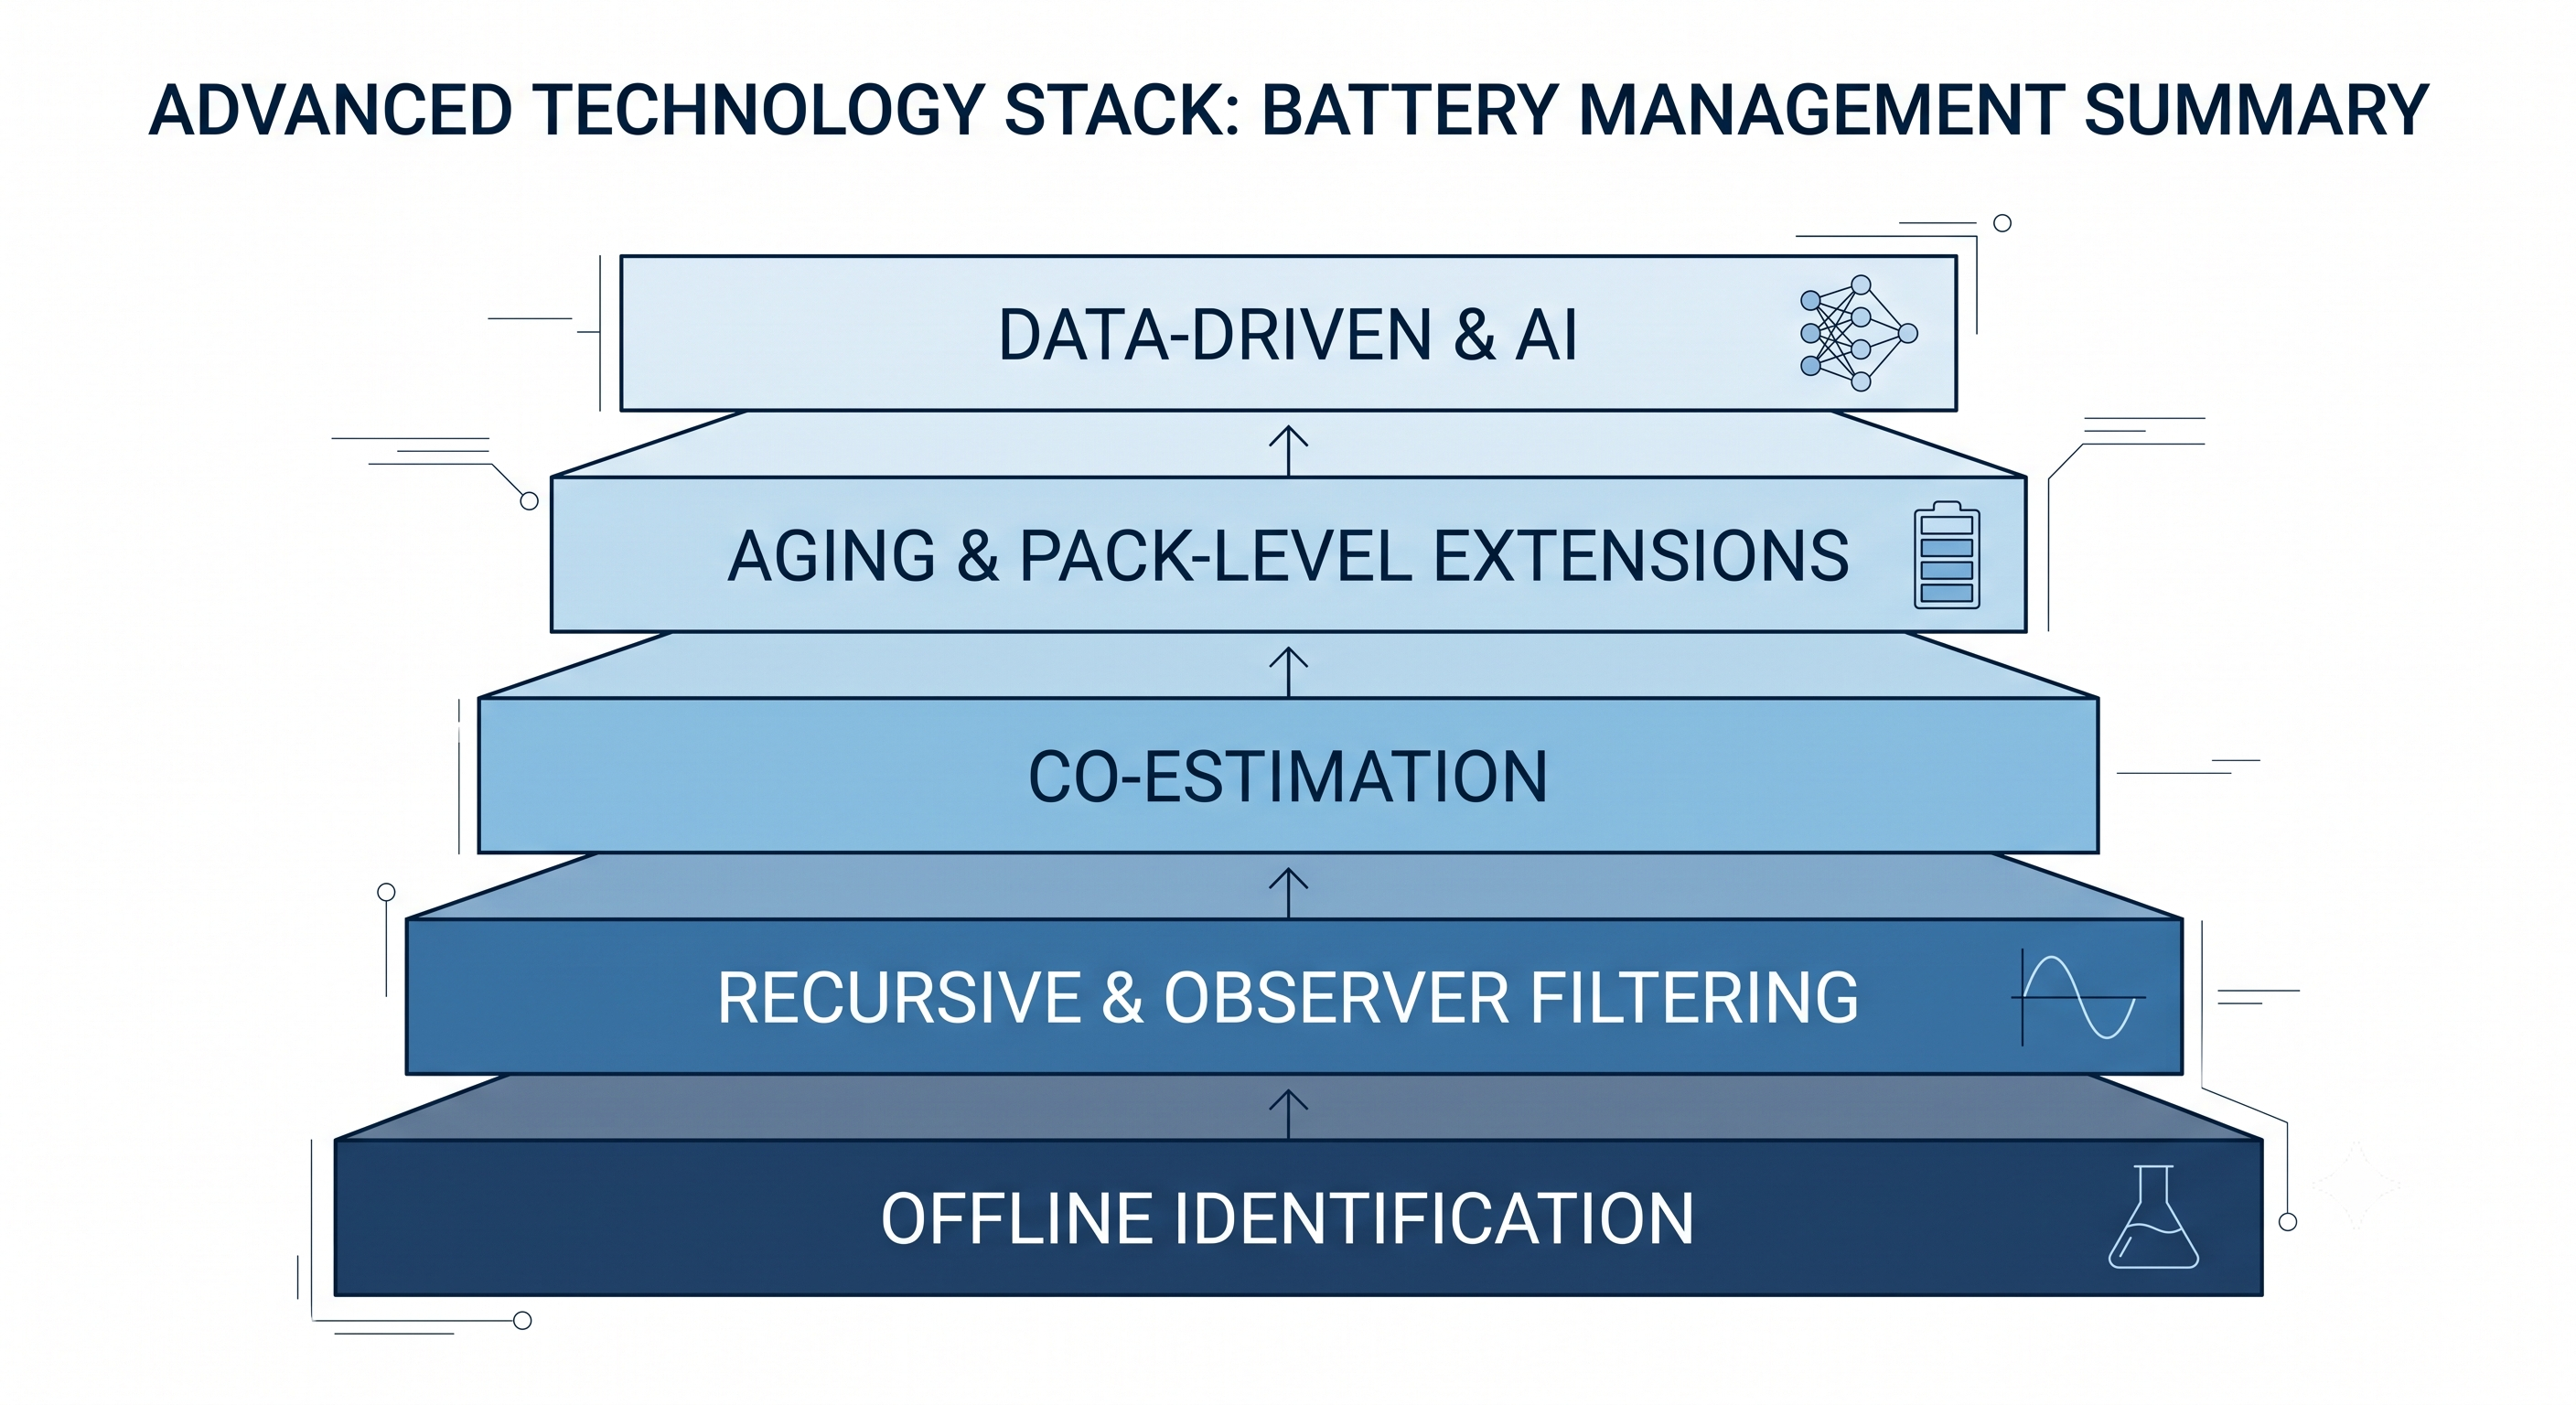
\includegraphics[width=0.9\textwidth]{ch-14-2.png}
\caption{Layered dependency structure of the estimation methodologies surveyed in this report.}
\label{fig:14_layered_architecture}
\end{figure}

% IMAGE PROMPT: A clean, editorial-style infographic summarizing a technology stack, drawn as a stack of horizontal layered blocks from bottom to top: "Offline Identification", "Recursive & Observer Filtering", "Co-Estimation", "Aging & Pack-Level Extensions", "Data-Driven & AI". Each block subtly connected by upward arrows indicating dependency, with small icons representing each layer (a lab flask for offline ID, a signal wave for filtering, a battery pack icon, a neural network icon). Minimalist technical report illustration style, blue and white color palette.

\section{Remaining Engineering Challenges in BMS Deployment}
\label{sec:14_remaining_challenges}

Despite continuous algorithm advancements, deploying these architectures into mass-market microcontrollers faces several physical, computational, regulatory, and organizational bottlenecks.

\subsection{Flat OCV Identifiability in Phase-Change Chemistries}
\label{subsec:14_flat_ocv}

In chemistries such as Lithium Iron Phosphate ($\text{LiFePO}_4$), the Open Circuit Voltage $V_{oc}(\text{SOC})$ derivative $\frac{d V_{oc}}{d \text{SOC}}$ approaches zero across $20\%$ to $80\%$ SOC. Within this plateau, terminal voltage measurements provide weak observability of SOC changes, making simultaneous state and parameter identification ill-conditioned. Resolving this requires excitation-gated updates or hybrid Ampere-hour tracking.

This challenge is compounded by the fact that LFP adoption in the broader EV market has been accelerating for cost and cobalt-supply reasons, meaning the very chemistry with the weakest voltage-based observability is simultaneously becoming one of the most commercially significant. As a result, hybrid strategies — combining coulomb counting as the primary SOC estimate with voltage-based correction reserved specifically for the steep regions near full charge and full discharge — have shifted from a specialized technique to something close to a default requirement for any LFP-based production BMS.

\subsection{Sensor Metrology and Non-Gaussian Noise}
\label{subsec:14_sensor_metrology}

Classical filtering algorithms assume zero-mean Additive White Gaussian Noise (AWGN). However, operational electric vehicles experience non-zero mean sensor offsets caused by thermal drift and electromagnetic interference (EMI) from inverter switching. Persistent current offsets induce unbounded integration errors if uncorrected:
\begin{equation}
\text{SOC}_{\text{err}}(t) = \int_0^t \frac{\eta \cdot I_{\text{bias}}}{3600 \cdot Q_{\text{nom}}} d\tau
\end{equation}

Beyond the steady-state bias captured by this equation, production current sensors (typically Hall-effect or shunt-based) also exhibit temperature-dependent gain error and, in Hall-effect designs specifically, hysteresis following large current transients — meaning the sensor's error is itself a function of the vehicle's recent usage history, not merely its instantaneous state. A rigorous BMS design must therefore characterize and compensate for a full sensor error model (offset, gain, temperature coefficient, and hysteresis) rather than treating the current sensor as an ideal, zero-error measurement channel, as is often implicitly assumed in academic treatments of the estimation algorithms themselves.

\subsection{Pack-Scale Computational Bottlenecks}
\label{subsec:14_pack_bottleneck}

As established in Chapter~11, automotive microcontrollers operate with strict RAM limits. While the Bar-Delta approach mitigates the $\mathcal{O}(d^3)$ EKF bottleneck, running comprehensive physics-based observers across 100+ series-connected cells while simultaneously managing active balancing duty-cycles pushes current embedded hardware to its absolute limit.

\subsection{Functional Safety Certification and Verification Burden}
\label{subsec:14_functional_safety}

A challenge largely orthogonal to raw computation, but no less significant in production timelines, is that any algorithm intended for deployment in a road vehicle's BMS must be verified and validated against automotive functional safety standards — most notably ISO~26262 — which impose stringent requirements on traceability, fault detection coverage, and deterministic worst-case execution time. Adaptive, data-driven components such as the LSTM and PINN architectures introduced in Chapter~8 pose a particular certification challenge: the "black box" nature of a trained neural network is difficult to reconcile with ISO~26262's expectation of traceable, analyzable failure modes, and the industry has not yet converged on a standardized methodology for certifying learned models to the same Automotive Safety Integrity Level (ASIL) rigor applied to traditional model-based observers. This gap between algorithmic capability and certifiability is, at present, one of the single largest obstacles preventing more aggressive adoption of the AI-based methods surveyed in Chapter~8 within safety-critical BMS software, as opposed to their more common current role as an offline, advisory diagnostic layer.

\subsection{Cybersecurity of Over-the-Air Parameter Updates}
\label{subsec:14_cybersecurity}

The Cloud-BMS and Digital Twin architectures discussed in Section~\ref{subsec:14_cloud_bms} depend on a continuous bidirectional data channel between the vehicle and a cloud backend, streaming telemetry upward and streaming updated parameter vectors and, in some architectures, updated model weights back down to the vehicle edge. This channel is, by construction, an attack surface: a compromised or spoofed parameter update could in principle cause a vehicle's BMS to systematically misestimate SOC or SOH, degrading performance or, in a worst case, undermining the safety margins the estimation stack is designed to preserve. Securing this channel requires cryptographic signing and integrity verification of every parameter update, secure boot and hardware root-of-trust on the vehicle-side microcontroller, and rollback protection to prevent an attacker from reverting a vehicle to a known-vulnerable older parameter set — requirements that sit outside the traditional scope of estimation theory but are inseparable from any real deployment of the cloud-connected architectures this chapter goes on to describe.

\subsection{Data Provenance, Fleet Heterogeneity, and Model Drift}
\label{subsec:14_data_provenance}

Every data-driven method surveyed in this report — from empirical fade-model fitting in Chapter~9 to the neural architectures of Chapter~8 — is only as trustworthy as the data used to build it. In practice, fleet data is heterogeneous by construction: vehicles are driven in different climates, charged on different infrastructure, and operated by drivers with very different behavioral patterns, meaning a model trained on an early-adopter fleet in a temperate climate may generalize poorly to a market with extreme heat or cold. Furthermore, as a given vehicle model's production hardware quietly evolves over its manufacturing lifetime (a different cell supplier, a revised busbar design, an updated current sensor part number), models trained on early-production data can experience \emph{silent drift} — a gradual divergence between the model's assumptions and the true population of vehicles it is being applied to, without any single dramatic failure event to trigger an obvious re-training alarm. Robust deployment requires ongoing model-performance monitoring against fleet ground truth, not a one-time training-and-deploy cycle.

\begin{table}[htbp]
\centering
\caption{Summary of remaining engineering and organizational challenges.}
\label{tab:14_challenges_summary}
\renewcommand{\arraystretch}{1.4}
\begin{tabularx}{\textwidth}{@{}l X@{}}
\toprule
\textbf{Challenge} & \textbf{Primary Risk if Unaddressed} \\
\midrule
Flat OCV identifiability & Poor SOC observability in LFP-dominant markets. \\
Non-Gaussian sensor noise & Unbounded SOC drift from uncompensated current bias. \\
Pack-scale computation & Inability to run full-fidelity per-cell observers within RAM/CPU budget. \\
Functional safety certification & Learned models blocked from safety-critical deployment. \\
Cybersecurity of OTA updates & Malicious or corrupted parameter updates degrading fleet-wide safety margins. \\
Data provenance \& fleet drift & Silently degrading model accuracy as fleet composition evolves. \\
\bottomrule
\end{tabularx}
\end{table}

\section{The Road Ahead: Next-Generation BMS Paradigms}
\label{sec:14_road_ahead}

To surmount computational, observational, regulatory, and security barriers, future battery management systems are evolving toward several core paradigms that build directly upon the foundations of Chapters 8, 9, and 11.


\subsection{Cloud-BMS and Digital Twin Architectures}
\label{subsec:14_cloud_bms}

Rather than executing heavy parameter estimation routines entirely on the edge, Cloud-BMS architectures offload non-real-time identification to cloud servers. Vehicle telemetry ($1\text{ Hz}$) is streamed via IoT connections to a cloud database maintaining a virtual ``Digital Twin.'' The cloud executes high-fidelity electrochemical models and SOH analytics to update slow aging parameters, streaming updated parameter vectors back to the vehicle edge for ultra-fast online tracking.

A critical, and often underemphasized, design constraint of this architecture is graceful degradation under connectivity loss: a vehicle operating in a region with poor cellular coverage, or simply parked in an underground garage, must continue to estimate SOC and SOH safely using its last-known-good parameter set, without any dependency on live cloud connectivity for core safety functions. The cloud layer should therefore be understood as an accuracy- and longevity-enhancing overlay on top of a fully self-sufficient edge estimation stack, not a replacement for it — a distinction that has direct implications for the functional-safety certification challenge discussed in Section~\ref{subsec:14_functional_safety}, since a certifiable safety function cannot, by definition, depend on an uncertifiable external network link.

\subsection{Relational Graph Convolutional Networks (R-GCNs) for Pack Topologies}
\label{subsec:14_gcn}

Standard neural networks struggle to map the spatial and thermal interactions of multi-cell packs. The next frontier in pack-level estimation models the battery module as a complex network graph, where cells are nodes and busbars/thermal pathways are edges. By applying Relational Graph Convolutional Networks (R-GCNs), a BMS can proactively predict localized hardware failures across the module. This enables advanced pack management strategies, such as automated traffic evacuation or dynamic electrical rerouting via software-defined networking paradigms, isolating failing cells before thermal runaway propagates.

The graph representation is a natural fit for the pack-level phenomena introduced in Chapter~11: the thermal-gradient feedback loop of Section~11.2, the parallel-group current skew problem, and the delta-filter divergence tracked by the Bar-Delta architecture are all, fundamentally, statements about relationships \emph{between} neighboring cells rather than properties of any single cell in isolation — precisely the structure a graph neural network is designed to exploit. Early research results suggest R-GCN-based approaches can anticipate localized imbalance formation several charge cycles before it becomes detectable by the scalar delta-filter thresholds described in Chapter~11, though translating this predictive lead time into an actionable, certifiable BMS intervention remains an open engineering problem.

\subsection{Fractional-Order Battery Modeling (FOM)}
\label{subsec:14_fom}

Traditional RC equivalent circuits rely on integer-order differential equations. However, porous electrode diffusion and SEI layer impedance exhibit continuous fractional dynamics. Fractional-Order Models replace standard capacitors with Constant Phase Elements (CPE):
\begin{equation}
I(t) = C_\alpha \frac{d^\alpha V_p(t)}{d t^\alpha}, \qquad 0 < \alpha < 1
\end{equation}
Fractional-order models capture mid-frequency impedance semicircles and diffusion tails with fewer parameters, achieving higher accuracy across wide temperature ranges.

The practical appeal of the fractional-order approach is parsimony: where a standard integer-order equivalent circuit model often requires two or three RC branches in series to adequately fit a cell's full impedance spectrum across the frequency ranges relevant to both fast transient response and slow diffusion-limited behavior, a single Constant Phase Element can frequently achieve comparable fitting accuracy with fewer free parameters. This parameter economy is attractive from an estimation standpoint (fewer parameters generally means better-conditioned, faster-converging online identification), but comes at the cost of requiring fractional-calculus-aware filter formulations — the standard EKF and UKF derivations of Chapters~5 and~7 assume integer-order state dynamics, and extending them rigorously to fractional-order systems remains an active area of applied mathematics research rather than a fully standardized, off-the-shelf technique.

\subsection{Edge AI Accelerators and On-Chip Neural Inference}
\label{subsec:14_edge_ai}

A complementary hardware-side trend to the cloud offload of Section~\ref{subsec:14_cloud_bms} is the increasing availability of dedicated neural processing units (NPUs) within automotive-grade microcontroller and system-on-chip designs. Where the data-driven and physics-informed methods of Chapter~8 were historically constrained by the limited floating-point throughput of conventional automotive MCUs, next-generation BMS silicon increasingly integrates small, low-power NPU cores specifically to run quantized inference for lightweight neural estimators directly at the edge, without requiring cloud round-trip latency. This trend does not eliminate the functional-safety certification challenge of Section~\ref{subsec:14_functional_safety} — a locally-executed neural network is no easier to formally verify than a cloud-hosted one — but it does substantially reduce the connectivity-dependence concerns of Section~\ref{subsec:14_cloud_bms}, and is likely to be the enabling hardware trend that eventually allows learned components to move from today's advisory, offline diagnostic role toward limited, tightly-bounded real-time deployment.

\subsection{Federated and Privacy-Preserving Fleet Learning}
\label{subsec:14_federated}

The data provenance and fleet heterogeneity challenge of Section~\ref{subsec:14_data_provenance} points toward a further architectural evolution: rather than centralizing raw vehicle telemetry in the cloud for model training — which raises both bandwidth costs and vehicle-owner data-privacy concerns — federated learning approaches train shared model updates locally on each vehicle's edge hardware and transmit only aggregated, privacy-preserving model gradients (rather than raw usage data) back to a central server for consolidation. This allows a fleet-wide degradation or fault-detection model to benefit from the full diversity of the fleet's operating conditions (directly addressing the heterogeneity concern of Section~\ref{subsec:14_data_provenance}) without requiring any single vehicle's detailed usage history to leave the vehicle in raw form, an increasingly important consideration as data-privacy regulation extends its reach into connected-vehicle telemetry.

\subsection{Second-Life and Circular-Economy Estimation Challenges}
\label{subsec:14_second_life}

Finally, as the first large generation of EV battery packs approaches automotive end-of-life (Chapter~9's $70$–$80\%$ $SOH_C$ threshold), a growing secondary application exists in repurposing these packs for stationary storage, where the acceptable SOH floor is typically much lower. This "second-life" context inverts several assumptions embedded throughout this report: the pack-level estimation architectures of Chapter~11 were designed around the expectation of a relatively fresh, well-matched string of cells, whereas a second-life pack is, by definition, composed of cells that have already diverged substantially and may originate from mixed production batches or even mixed vehicle models during pack reconditioning. Estimation architectures for second-life applications must therefore be re-validated against a starting population with far greater baseline heterogeneity than the fresh-pack scenario implicitly assumed by most of the algorithms surveyed in Chapters~4 through~13, representing a distinct and still-maturing sub-field of battery management research.

\begin{figure}[htbp]
\centering
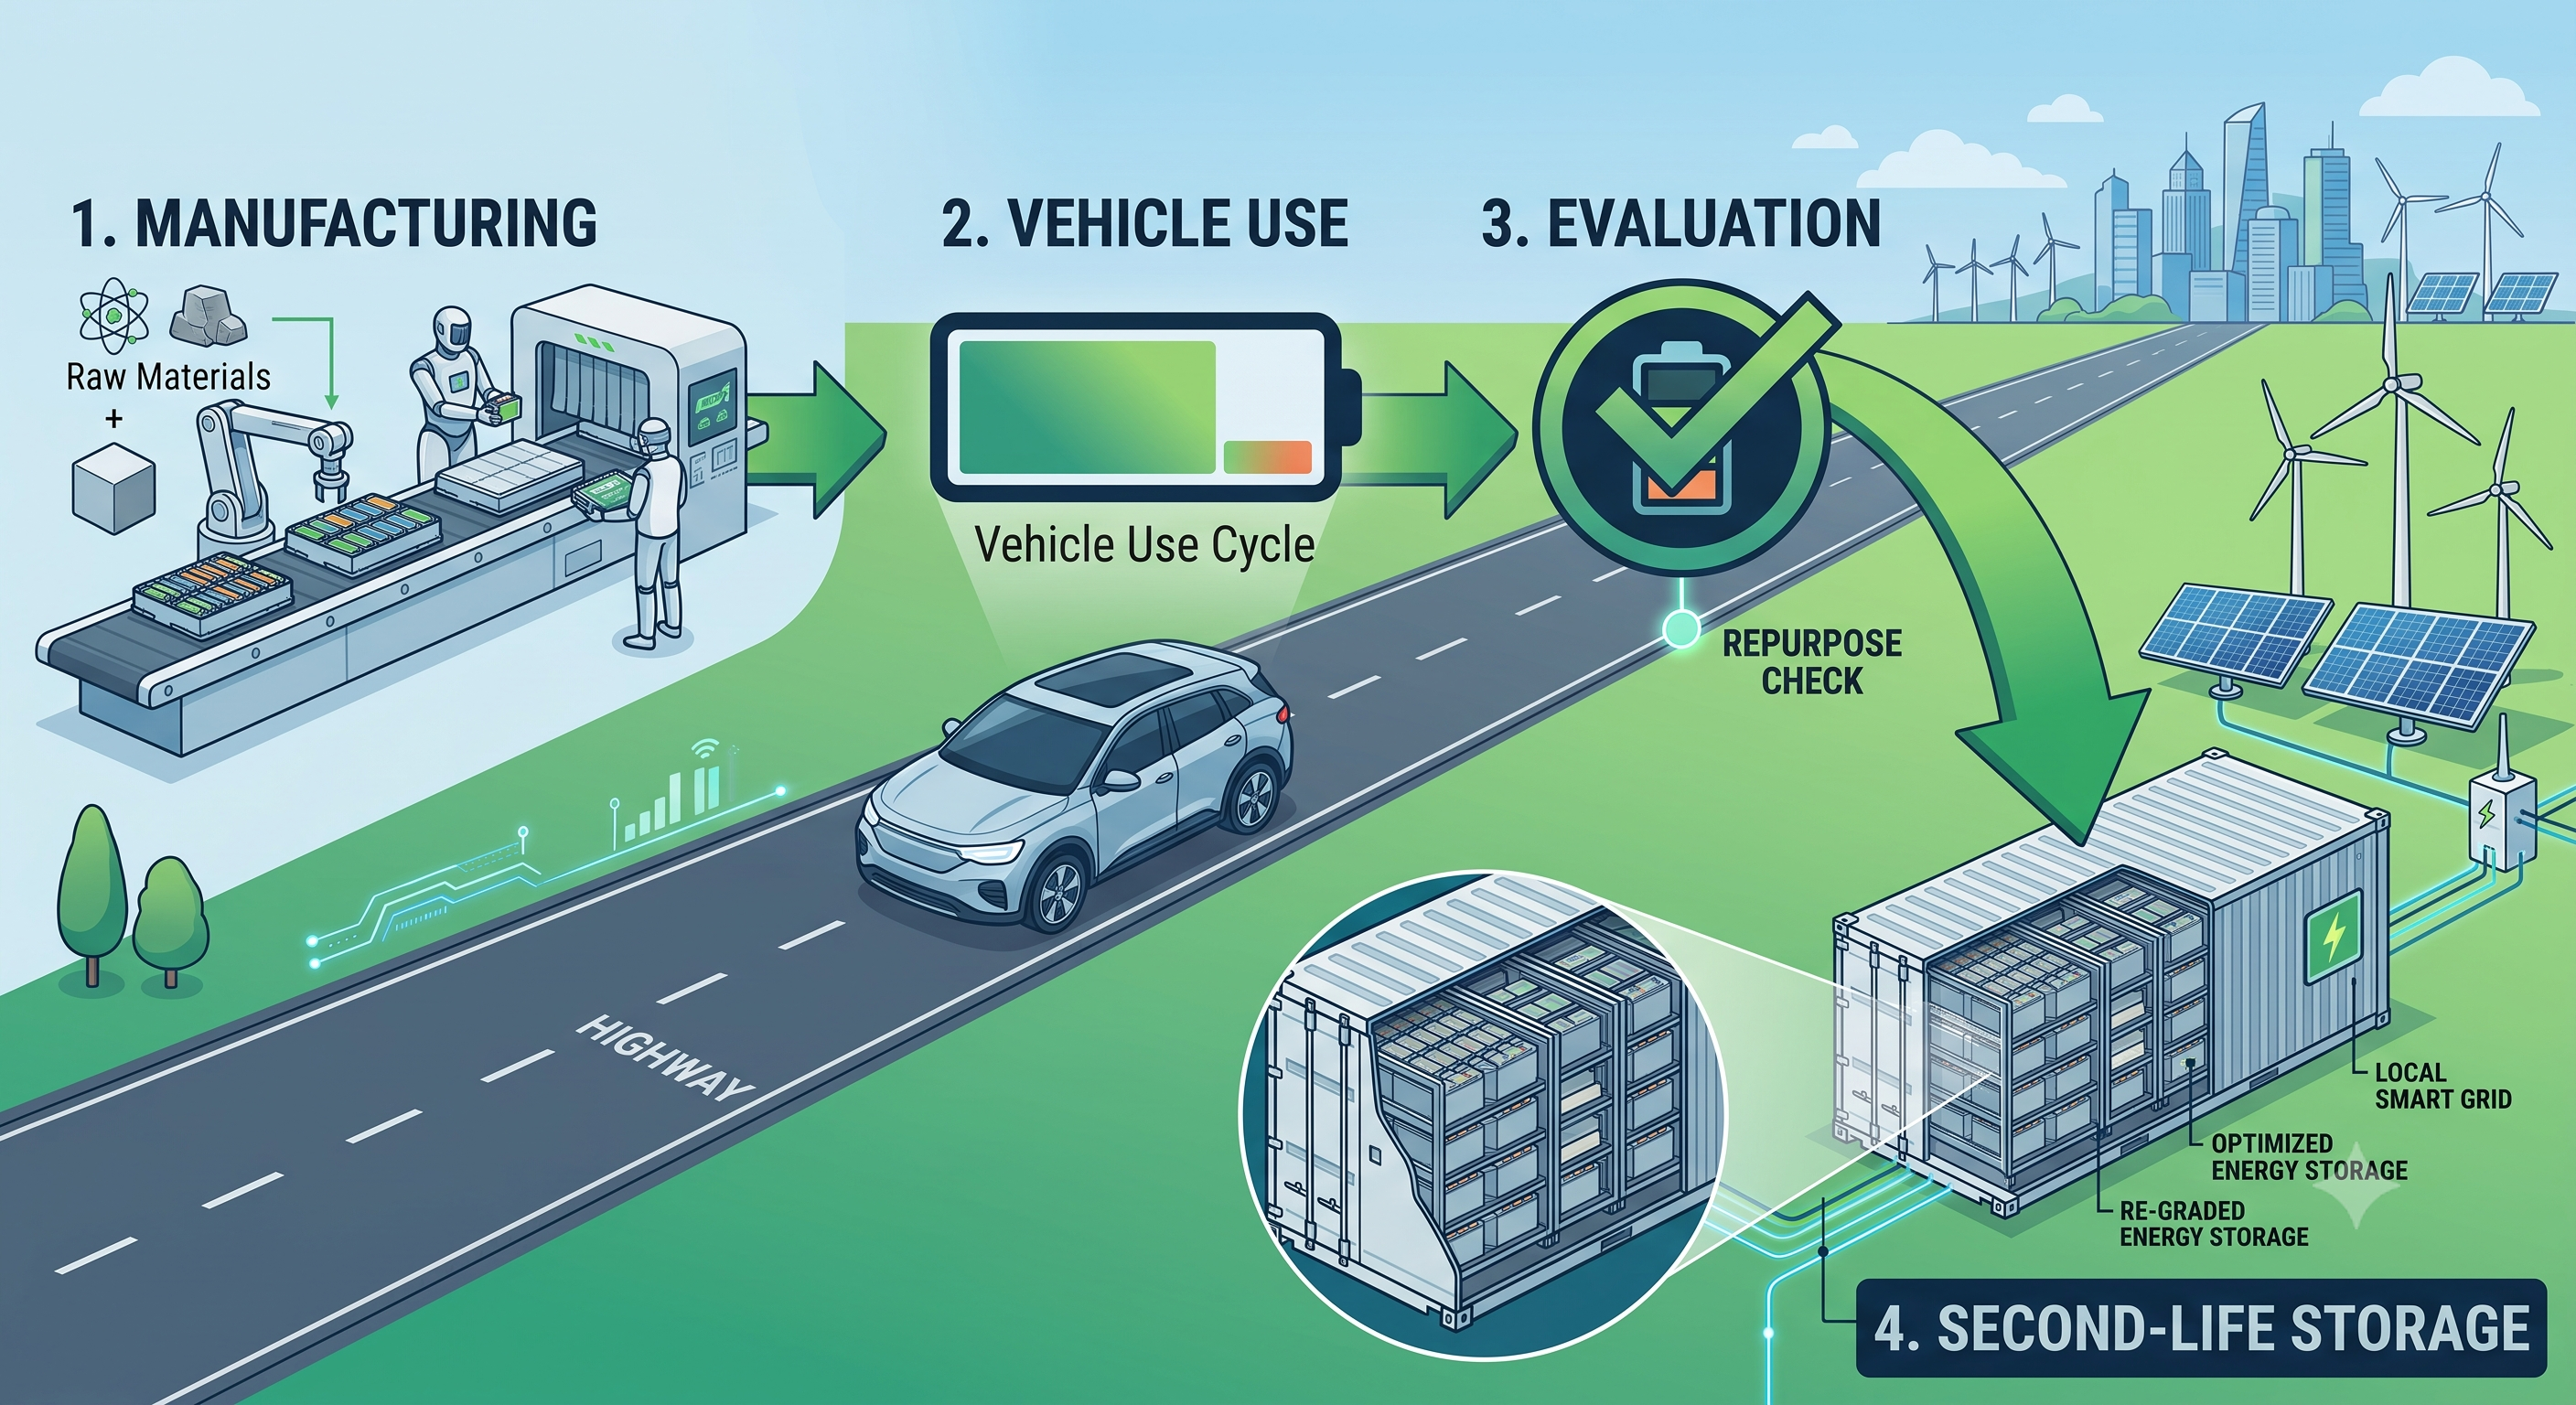
\includegraphics[width=0.65\textwidth]{ch14-1.png}
\caption{Conceptual technology adoption roadmap for next-generation BMS paradigms.}
\label{fig:14_roadmap_placeholder}
\end{figure}

% IMAGE PROMPT: A futuristic circular economy infographic illustration showing an electric vehicle battery pack's lifecycle: manufacturing, first-life vehicle use with a Bar-Delta estimation icon, end-of-life threshold marker, then an arrow curving toward a "second-life" stationary storage container installation with a distinct, more heterogeneous cell-icon pattern. Clean vector illustration, green and blue sustainability-themed color palette, engineering-report style.

\section{Summary of Open Research Questions}
\label{sec:14_open_questions}

Drawing together the challenges and emerging paradigms discussed above, Table~\ref{tab:14_open_questions} distills the report's findings into a concise list of open research questions most likely to shape the next generation of battery management scholarship and product development.

\begin{table}[htbp]
\centering
\caption{Open research questions arising from this report.}
\label{tab:14_open_questions}
\renewcommand{\arraystretch}{1.4}
\begin{tabularx}{\textwidth}{@{}l X@{}}
\toprule
\textbf{Theme} & \textbf{Open Question} \\
\midrule
Certifiable AI & How can learned (neural or fractional-order) estimators be verified to automotive ASIL rigor without sacrificing their accuracy advantages? \\
Pack-scale graph models & Can R-GCN-based imbalance prediction be translated into a bounded, real-time, certifiable BMS intervention? \\
Federated fleet learning & What aggregation and privacy-preservation schemes best balance fleet-wide model quality against per-vehicle data privacy? \\
Second-life reuse & How must Bar-Delta and balancing architectures be re-designed for pack populations with substantially higher baseline heterogeneity? \\
Cybersecurity & What minimal, provably-secure update protocol is sufficient to protect cloud-to-edge parameter streaming without excessive latency overhead? \\
\bottomrule
\end{tabularx}
\end{table}

\section{Concluding Remarks}
\label{sec:14_summary_conclusion}

Parameter estimation is the bridge between physical battery electrochemistry and cyber-physical control. Across the thirteen preceding chapters, this report has traced that bridge from its foundations — static offline curve fitting against a single equivalent circuit — through the recursive, adaptive, and observer-based techniques that allow a real vehicle to track its own internal state in real time, through the aging and pack-level extensions required to account for the fact that a battery is neither a fixed nor a solitary object, and finally to the data-driven and physics-informed methods that are beginning to blur the line between explicit electrochemical modeling and learned representation.

No single algorithm surveyed in this report is sufficient on its own; production-grade battery management is, and will likely remain, an integration exercise across offline calibration, online adaptation, pack-scale coordination, and — increasingly — cloud- and fleet-scale learning, bound together by the functional-safety and cybersecurity discipline required of any system entrusted with the energy storage backbone of a moving vehicle. As battery technology itself continues to evolve — toward silicon-anode and eventually solid-state chemistries, toward higher energy densities and faster charge acceptance, and toward a genuinely circular second-life economy — the estimation architectures documented in this report will themselves need to evolve in parallel. The integration of fractional-order models, physics-informed neural networks, graph-based spatial topologies, edge AI acceleration, and cloud/federated digital twins outlined in this concluding chapter represents not a finished destination, but the current leading edge of a field that will continue to unlock greater energy efficiency, safer rapid charging, and extended operational lifespan for the energy storage systems that underpin the broader transition toward electrified transportation and grid infrastructure.

No single algorithm surveyed in this report is sufficient on its own; production-grade battery management is, and will likely remain, an integration exercise across offline calibration, online adaptation, pack-scale coordination, and — increasingly — cloud- and fleet-scale learning, bound together by the functional-safety and cybersecurity discipline required of any system entrusted with the energy storage backbone of a moving vehicle. As battery technology itself continues to evolve — toward silicon-anode and eventually solid-state chemistries, toward higher energy densities and faster charge acceptance, and toward a genuinely circular second-life economy — the estimation architectures documented in this report will themselves need to evolve in parallel. The integration of fractional-order models, physics-informed neural networks, graph-based spatial topologies, edge AI acceleration, and cloud/federated digital twins outlined in this concluding chapter represents not a finished destination, but the current leading edge of a field that will continue to unlock greater energy efficiency, safer rapid charging, and extended operational lifespan for the energy storage systems that underpin the broader transition toward electrified transportation and grid infrastructure.